\section{Introduction}

\label{sec:intro}

Since the advent of the Information Age, data collection and analysis have become more and more essential to modern life. The need for fast processing of enormous volumes of data has stimulated exciting innovations in information technology infrastructure. In particular, distributed processing, also known as grid computing, has emerged as an efficient means of processing large scale data by distribution of the workload over a large network of individual processing units.\\ 

On the other hand, procuration of such a large number of processing units requires funds and infrastructure typically available only to governments, corporations, and universities. In a competitive funding environment, organizations and individuals with valuable data to process may nevertheless end up excluded from traditional funding channels. Even projects of significant and fundamental interest to humanity may fall under this category, due to their inability to satisfy government and corporate interests or secure short-term monetary returns. \\

Perhaps surprisingly, however, the means to circumvent this barrier are already on hand, sitting on our desks at home or lodged in our pockets: The combined Idle Processing Potential (IPP) of consumer electronic devices overshadows even the most robust decentralized super-computer, Bitcoin. Nevertheless, IPP is severely underutilized. To tap into this potential, Gridcoin seeks to create a decentralized and sustainable distributed processing network which prioritizes both the utilization of IPP and the creation of a free host ecosystem for researchers and individuals with data to process. Towards this end, Gridcoin has created a blockchain-based digital asset which rewards individuals and entities which volunteer their IPP to the grid computing network, BOINC.  A single Gridcoin represents the value prescribed to a volunteered unit of IPP on the BOINC network.  The Gridcoin blockchain is secured through Proof of Stake.  Rewards are distributed through a protocol developed by Gridcoin called Distributed Proof of Research, or DPoR.\\

\begin{figure}
\centering
\includegraphics{figures/Gridcoin-art-small}
\medskip
\caption{\textit{Gridcoin Art Medal depicting research in the fields of biology, electronics and astrophysics}}
\small
\end{figure}

BOINC, The Berkeley Open Infrastructure for Network Computing, is an open source distributed processing network which provides scientists and enthusiasts with means to process computational data for free. In operation since 2002, BOINC has maintained an active community consisting of hundreds of thousands of users. This vast userbase reliably contributes the computational muscle to support a wide range of independent projects, such as mapping the Milky Way galaxy, finding record prime numbers, folding proteins, testing disease cures and vaccines, and searching for extraterrestrial life.\\

By directly rewarding those who volunteer their idle processing power to BOINC, Gridcoin creates an ecosystem in which valuable data, or a worthwhile project, is defined by an "open market of science" instead of a market of "pay-to-play".  In other words, volunteers will move their IPP to projects in which they find intrinsic value. This eliminates the bias towards the researchers and organizations who happen to have the most funding.\\

A typical node on the Gridcoin network runs two clients: 1) the BOINC client, which manages the downloading and processing of data, and 2) the Gridcoin client, which interfaces with other nodes on the Gridcoin network. Like a Bitcoin wallet, the Gridcoin client allows users to transfer money to and from different addresses. Moreover, it contributes to the overall health of the network by verifying each new block and, depending on the configuration, itself staking new blocks. The coinstake in the new blocks proposed by any given wallet corresponds to an associated amount of work done on BOINC, expressed in Gridcoins.\\

\subsection{BOINC}

BOINC users run a client which downloads and manages the processing of work units (WU) for specific projects. A work unit consists of executable code and specific parameters for which the code is run.  After the work unit is completed the BOINC client returns the results to the BOINC servers.

An example BOINC project is the World Community Grid [11], which is composed of various research initiatives with a humanitarian focus, for instance fighting cancer or curing Ebola. SETI@home [20], which scans radio waves from space for signs of alien life, is another well-known project.  In total there are over 40 BOINC projects, but only the BOINC projects on the Whitelist help users earn Gridcoins. The complete Whitelist is available in the appendix. Each Gridcoin wallet can vote in polls concerning which projects enter or exit the Whitelist. New projects with interesting computational tasks have a high chance of getting on the Whitelist, while projects which do not have a constant supply of work units tend to be dropped. \\

The computational output of a given Gridcoin user is measured and stored on the BOINC server. The unit of work is a cobblestone, which on a project-by-project basis is converted into a certain number of "credits".  While credits accumulate over time, computational \textit{power} is measured by the Recent Average Credit (RAC), defined as a weighted time-average of credits earned per unit time. These units of measure are discussed later on in this whitepaper.\\

A CPID (Cross Project Identifier) is a unique identifier on the BOINC network that links the contributions of a single user to different projects. Knowledge of a user's CPID allows anyone to view the contributions of that user to BOINC projects.\\

Finally, BOINC also allows the creation of teams. When a user joins a team, the work done by that member is added to the total work done by the team. To earn Gridcoin, a user must join team \textit{Gridcoin}, which on some projects is listed as \textit{gridcoin}, lowercase.

\begin{figure}
\centering
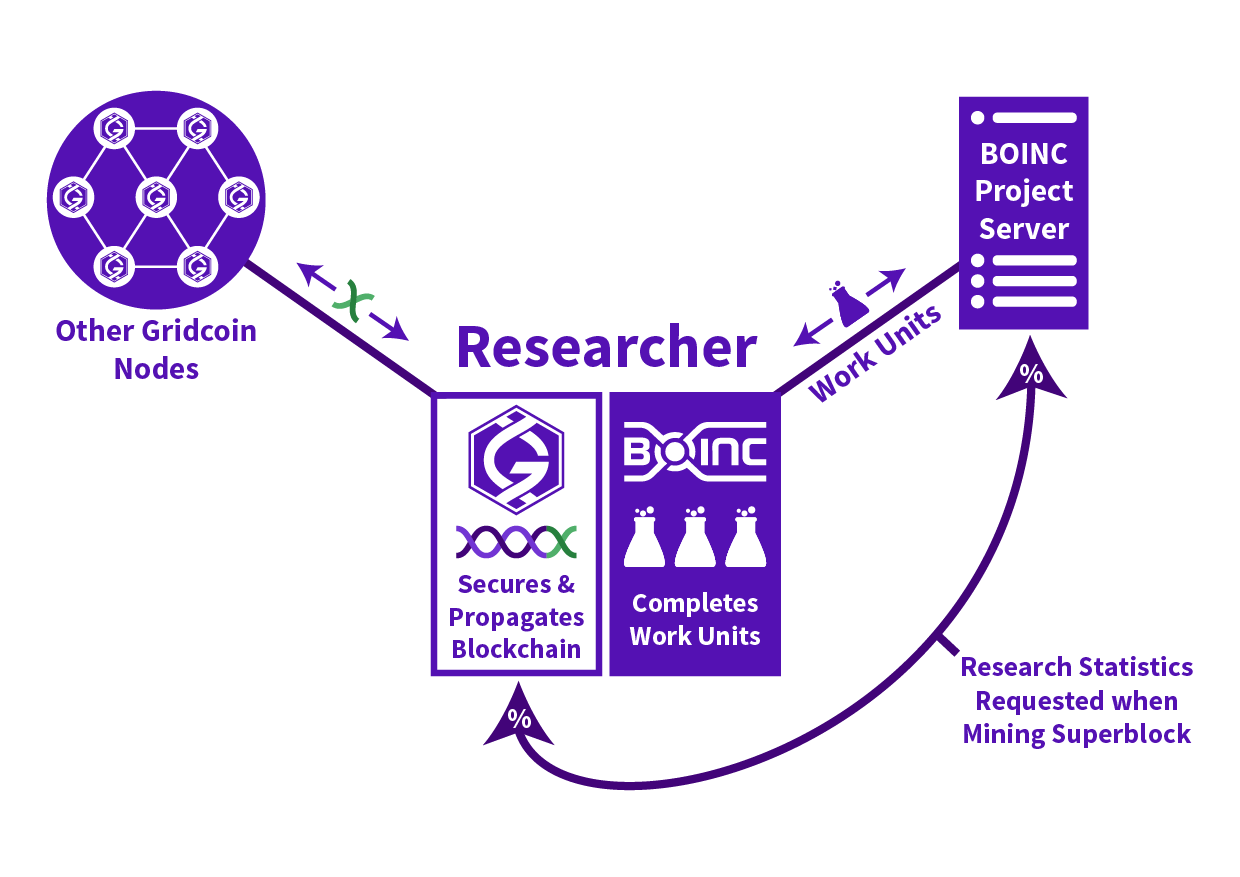
\includegraphics[scale=0.5]{figures/researcherdiagram_joshoeah}
\medskip
\caption{\textit{Gridcoin and BOINC Architecture} [5]}
\small
\end{figure}

\subsection{Gridcoin Client}

The Gridcoin Client is very similar to a Bitcoin client, inheriting substantial portions of source code from it. It is sometimes called a wallet, because it stores the Gridcoins owned by a user. The client allows users to receive and send Gridcoins to other clients. If it is attached to BOINC, it is able to mine blocks which reward the user for work done on BOINC. The client also occasionally stakes Gridcoins so that they earn interest.

\subsection{Setting Up a Network Node to Earn Gridcoins}

Tutorials for setting up BOINC and the Gridcoin client are available on www.gridcoin.us. Briefly, the steps to become a solo miner are as follows:
\begin{enumerate}
  \item Install BOINC.
  \item Add projects to BOINC that belong to the Whitelist [42].
  \item Install and configure the Gridcoin wallet so that it is linked to BOINC.
  \item Acquire Gridcoins by buying them on exchanges and transferring them to your wallet.
  \item Send a beacon so that the wallet CPID is present in the blockchain.
\end{enumerate}
With proper setup, the client can begin staking blocks and rewarding the miner with Gridcoin. The odds of staking a block are proportional to the number of coins owned; the expected time until the next block is staked can be estimated from within the client. Note, however, that this is only an estimate of the average: the actual time to stake a block may be smaller or larger.

On the aforementioned website there are also instructions about mining in a common pool, which in contrast with solo mining has the advantage of consistent and predictable payouts. There is also the possibility to be an \textit{investor} simply by owning Gridcoins and running the Gridcoin client (without needing to be a BOINC researcher). In the latter case, the investor earns interest on the Gridcoins they own, simply by running the wallet.\\

\subsection{Mining Pool}

If users do not manage to get some starter coins, available from faucets, or if they lack the experience to buy them from exchanges, they have the possibility to join the Gridcoin Mining Pool [55]. Steps to become a pool miner are as follows:

\begin{enumerate}
  \item Register with GRCpool.com and select projects in which to participate.
  \item Install BOINC.
  \item Add GRCpool as account manager in BOINC. BOINC will download the selected projects in step 1. BOINC will submit computed results under the CPID of GRCpool. Thus, GRCpool will credit the user's balance on the website depending on how much work was performed. 
  \item Install the Gridcoin wallet in investor mode, without linking it to BOINC. Create a new Gridcoin address.
  \item Login into GRCpool.com and move the credited Gridcoins to the local wallet by using the newly created Gridcoin address
\end{enumerate}

Mining with the pool is easier to setup, but has two main drawbacks. First, the user does not inherit his/her own BOINC statistics. Instead, these are formally credited to the mining pool. Second, the user is not able to vote in polls issued by the network (see chapter 9).

\subsection{Mining on Several Devices}

Independent of whether the user mines solo or in the pool, it suffices to set up a single Gridcoin wallet linked to the same BOINC credentials. All devices used for mining will install BOINC and use the same credentials. Currently it is possible to mine Gridcoin using cell phones, tablets, PCs (even Raspberry Pi and its clones), playstations, high end servers, and advanced mining equipment. Both CPU and GPU mining are available, depending on the project.

In the foreseeable future, this list may expand further. With the growth of the Internet of Things, mining may even become possible on devices such as smart watches and house appliances! 

\subsection{Integrating Gridcoin in Existing Exchanges}

For exchanges that wish to integrate Gridcoin in their infrastructure, the client can be run entirely in textual mode out of a Linux bash shell. The daemon named \textit{gridcoinresearchd} implements the same commands with the same syntax as \textit{bitcoind}, making the integration of Gridcoin in any existing cryptocurrency exchange infrastructure quick and easy [56].\\
